\documentclass[times, utf8, diplomski, numeric]{fer}
\usepackage{booktabs}

\usepackage{float} % "place table exactly here" package

\usepackage{listings}

\begin{document}

\thesisnumber{1954}

\title{Stvarnovremensko praćenje parametara ispravnosti rada u sustavu za raspodijeljenu obradu tokova podataka}

\author{Mislav Jakšić}

\maketitle

\izvornik

\zahvala{Hvala svima!}

\tableofcontents

\chapter{Uvod}

Raspodijeljeni sustavi su nepouzdani. Pogreška u sklopovlju, operacijskom sustavu, programu ili mreži može izazvati ispad bilo kojeg dijela sustava. Ispadi u raspodijeljenom sustavu mogu pokrenuti lanac ispada. Ako ispad ne uzrokuje lanac ispada sustav će i dalje patiti jer će program i dalje zahtijevati računalno vrijeme i memoriju, a s njima neće obavljati koristan posao. U najgorem slučaju ispad može izazvati potpuno zatajenje sustava gdje je jedini lijek iznova pokrenuti sve njegove dijelove. U najboljem slučaju ispad će samo smanjiti učinkovitost sustava. Bez pažljivog nadzora raspodijeljenog sustava teško je otkriti ispad, a još teze otkloniti izvor ispada.

Zadatak nadzora je otkriti ispad i njegov uzrok. \citep{rassus-manual} ispade dijeli na ispad procesa, pogreške u komunikaciji, vremenske pogreške, pogrešan odgovor i bizantske pogreške. Ako se ispad želi otkriti potrebno je pratiti vrijednosti koje ukazuju da se ispad dogodio. Korisne vrijednosti mogu biti zauzeće memorije, brzina obrade zahtjeva, sadržaj poruke ili duljina uspostave komunikacijskog kanala. Nadzirani program vrijednosti predaje nadzorniku koji je čovjek ili program. Ako nadzor obavlja program on treba biti pouzdaniji od nadziranog programa inače je problem nadzora udvostručen, a ne riješen.

Prvi korak u izradi pouzdanog sustava nadzora je izrada pouzdanog sakupljača vrijednosti. Prije same izrade istražene su ideje, sukobljene su arhitekture i uspoređena postojeća rješenja. Kako bi naglasak na idejama, arhitekturama i izradi rješenja bio podjednak napravljen je sakupljač za jedan raspodijeljeni sustav. Kada bi umjesto njega bio napravljen svestran sakupljač koji može sakupljati vrijednosti raznolikog sklopovlja, operacijskih sustava i programa misli o arhitekturi bile bi izražene na uštrp onima o izradi programa. Nadzirani sustav je Apache Kafka, popularni sustav za raspodijeljenu obradu tokova podataka.

\chapter{Sustavi za raspodijeljenu obradu tokova podataka}

\citep{ilprints535} razlikuje tok podataka od skupa podataka. Toku podaci dolaze stalno, u nepoznatom redoslijedu, bez znaka kada će prestat i bit će odbačeni nakon što su pročitani. Ovi sustavi su raspodijeljeni jer se tok mora obraditi brzo. Primjer problema toka podatka su kartično plaćanje, praćenje korisnika mrežnih stranica, posluživanje reklama i preporuka. Svi navedeni problemi imaju mnogo izvora i ponora podataka. Kako sakupiti, zabilježiti, te dostaviti podatke na ponor gdje će se obraditi su problemi za koje sustavi za raspodijeljenu obradu tokova podataka nude rješenje. Zato što su tokovi podatka raznovrsni razvijeno je mnoštvo alata za njihovu obradu. Alate razlikujemo po načinu sakupljanja podataka, po mogućnostima toka, po arhitekturi i načinu zapisivanja podataka.

Prije razvoja sakupljača vrijednosti potrebno je usporediti i izabrati alat za raspodijeljenu obradu podataka. Kako bi usporedba alata i izvedba sakupljača bila jednostavnija u obzir su uzeti samo javno dostupni alati. Većina takvih alata koristi model objavi/pretplati. Umjesto da se usporede svi javno dostupni alati izabran je predstavnik iz svakog važnog skupa alata:
\begin{itemize}
    \item Apache Kafka je predstavnik popularnih alata za raspodijeljenu obradu tokova podataka
    \item Apache Pulsar je predstavnik modernih alata. \citep{yahoo-blogpost} je 2016. objavio Pulsar dok je \citep{kafka-whitepaper} objavio Kafku 2011. godine
    \item RabbitMQ je predstavnik alat koji potiskuju podatke prema korisnicima. Za razliku od RabbitMQ korisnici Kafke i Pulsara moraju povlačiti podatke
\end{itemize}

\section{Model objavi/pretplati}

\begin{figure}[H]
    \centering
    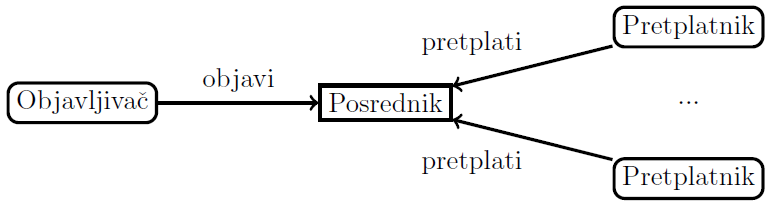
\includegraphics[width=0.8\textwidth]{PublishSubscribe.png}
    \caption{Model objavi/pretplati}
    \label{fig:publish-subscribe}
\end{figure}

Apache Kafka, Apache Pulsar i RabbitMQ koriste model objavi/pretplati za razmjenu podataka između procesa. \ref{fig:publish-subscribe} prikazuje nužne dijelove modela objavi/pretplati. \citep{rassus-manual} navodi da se model objavi/pretplati sastoji od objavljivača koji šalju poruke, pretplatnika koji čitaju poruke i posrednika koji razmjenjuje poruke između njih. Posrednik zapisuje objavljene poruke i dopušta pretplatnicima da ih čitaju. Prednost modela objavi/pretplati nad izravnim razgovorom među procesima je što objavljivači i pretplatnici ne trebaju znati jedan za drugoga.

\section{Apache Kafka}

\begin{figure}[H]
    \centering
    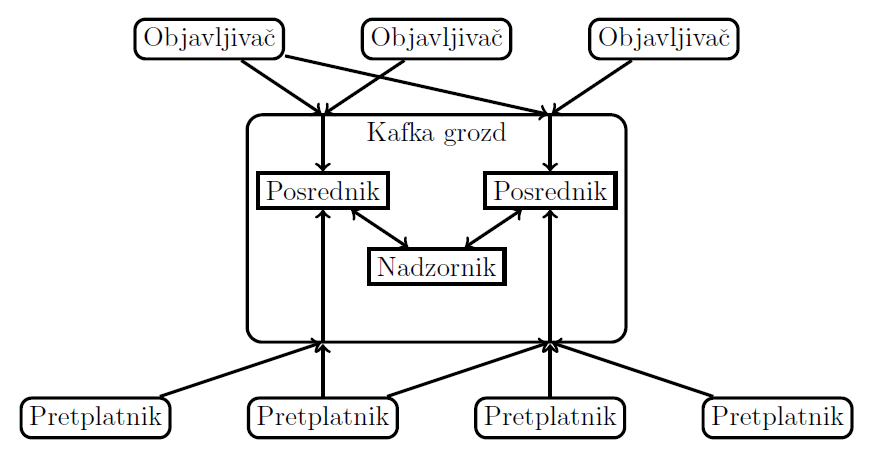
\includegraphics[width=0.8\textwidth]{KafkaCluster.png}
    \caption{Apache Kafka grozd}
    \label{fig:kafka-cluster}
\end{figure}

Apache Kafka je popularni alat za raspodijeljenu obradu tokova podataka. \ref{fig:kafka-cluster} prikazuje Kafka grozd. Svaki grozd sastoji se od ZooKeeper nadzornika i barem jednog posrednika. Nadzornik usklađuje posrednike. Objavljivači šalju poruke u temu grozda. Posrednici zapisuju poruke u pretinac teme. Pretplatnici čitaju poruke iz teme grozda i obrađuju podatke. \citep{kafka-whitepaper} \citep{kafka-docs} opisuju primjenu, arhitekturu i izvedbu Kafka pretplatnika, pretinca, posrednika, teme i objavljivača.

\subsection{Objavljivač}
Objavljivač je korisnički program koji šalje poruke u temu grozda. Poruka se nužno sastoji od sadržaja, teme na koju se objavljuje, oznake pretinca, odmaka u pretincu i vremena objave. Poruke se šalju u skupini nakon sto prođe određeno vrijeme ili se nakupi dovoljno poruka. \cite{kafka-compression} navodi kako poruke sažeti prije slanja. Tema je podijeljena na pretince. Pretinac je dnevnik u koji posrednik zapisuje poruke. Posrednik je poslužitelj koji zapisuje poruke u pretinac. Objavljivač ili ključem izabere pretinac u koji želi zapisati poruke ili se poruke šalju u svaki pretinac jednoliko. Posrednik će poslati potvrdu kada se poruke zapišu u pretinac vođe i izabrani broj usklađenih sljedbenika. Prije slanja sljedećeg skupa poruka objavljivač može pričekati potvrdu posrednika.

Ako se dogodi ispad objavljivača ili posrednika, objavljivač će ponovno poslati poruke. Objavljene poruke biti će dostavljene posredniku barem jednom. Ako je uvišestručavanje poruka nedopustivo, objavljivač može koristiti transakcijski način rada.

\subsection{Tema}
Tema je tok poruka, apstraktna umotvorina u koju objavljivači šalju poruke, a iz koje pretplatnici čitaju poruke. Posrednici se brinu da poruke budu zapisane. Biti pretplaćen na temu znači napraviti podtok poruka. Poruke objavljene u temu se ravnomjerno raspoređuju u podtokove. Svaki podtok ima pokazivač kojim pretplatnik čita poruke. Ako pokazivač dođe do kraja podtoka, pretplatnik se blokira dok se ne objavi nova poruka. Količina nepročitanih poruka u temi ne utječe na protok poruka kroz temu. Poruke u temi se brišu tek nakon određenog vremena. Tema je podijeljena na pretince s kojih posrednici čitaju i u koje pišu poruke. Kako bi poruke u pretincu bile dostupne nakon ispad posrednika, pretinac je moguće umnožiti.

\subsection{Posrednik}
Posrednik je poslužiteljski program koji zapisuje poruke objavljivača i poslužuje poruke pretplatnicima. Svaki posrednik dio je samo jednog Kafka grozda. Posrednici koriste Apache ZooKeeper za izvršavanje sporazumnog algoritma, pamćenje tema, njihovih pretinaca i usklađenih posrednika. Posrednik će poruke zapisati u pretinac onim redoslijedom kojim je objavljivač poslao poruke, ne redoslijedom kojim je posrednik primio poruke. Pretplatnici će s posrednika čitati poruke onim redoslijedom kojim su zapisane u pretinac.

Kada objavljivač objavi poruke na temu posrednik će zapisati poruke u određeni pretinac. Posrednik koristi sustav straničenja i tvrdi disk za zapisivanje poruka opisano u \cite{kafka-paging}. Umjesto da posrednik koristi memoriju procesa za priručnu memoriju posrednik poruke predaje sustavu straničenja operacijskog sustava. Operacijski sustav će poruke zapisati u stranice i pohraniti u nedodijeljene dijelove radne memorije. Poruke se zapisuju na tvrdi disk samo kada operacijski sustav želi osloboditi memoriju sustava straničenja. Opisano gospodarenje memorijom dopusta posredniku da čuva veliku količinu poruka bez gubitka učinkovitosti.

Pretplatnici često dohvaćaju uzastopne poruke pa se one čitaju iz priručne memorije umjesto iz tvrdog diska. Zahvaljujući sustavu straničenja priručna memorija sa zapisanim porukama će postojati neko vrijeme nakon ispada posrednika. Korištenjem sustava straničenja za zapisivanje poruka izbjegava se korištenje sakupljača smeća Java virtualnog stroja. Umjesto da se poruke zapisu dva puta, jednom u dodijeljenu memoriju procesa i jednom u sustav straničenja poruke se zapisu samo jednom u sustav straničenja.

Kada pretplatnik želi pročitati poruke posrednik će pronaći, pročitati i poslati poruke pretplatniku. \cite{linux-sendfile} \cite{java-zero-copy} opisuju kako posrednik s sendfile i zero-copy funkcijama čita poruke iz radne memorije i šalje u memoriju mrežne kartice u jednom koraku. Kako bi se dodatno ubrzao rad posrednici, objavljivači i pretplatnici grupe poruka čitaju, zapisuju i šalju u istom binarnom obliku. Prije slanja poruka pretplatnicima posrednik može sažeti poruke.

\subsection{Pretinac}

\begin{figure}[H]
    \centering
    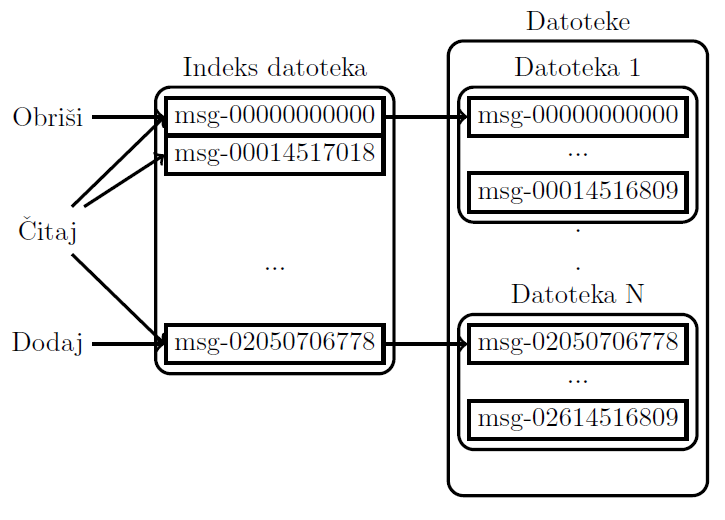
\includegraphics[width=0.8\textwidth]{KafkaLog.png}
    \caption{Kafka dnevnik}
    \label{fig:kafka-log}
\end{figure}

Pretinac je logički dnevnik i najmanja gradivna jedinica teme. Kada objavljivač objavi poruku u temu grozda posrednik poruke zapiše u pretinac teme. \ref{fig:kafka-log} prikazuje dnevnik izveden kao skup datoteka iste veličine. Kada posrednik zapiše poruke u pretinac on doda poruke na kraj datoteke. Datoteke se predaju sustavu straničenja operacijskog sustava tek nakon određenog vremena ili broja dodavanja. Svaka poruka ima jedinstvenu oznaku koja je ujedno i odmak unutar datoteke. Odmak sljedeće poruke računa se kao zbroj odmaka i veličine ranije poruke. Zato su oznake poruka jedinstvene i strogo rastuće ali nisu uzastopne.

Protok poruka kroz temu može biti toliki da izazove preopterećenje posrednika. Zato je temu moguće podijeliti na više pretinaca. Ako je B broj posrednika u Kafka grozdu onda tema može biti podijeljena na najviše B pretinaca. Svaki pretinac teme mora biti dodijeljen različitom posredniku.

Ako se dogodi ispad posrednika, poruke u pretincu postat će nedostupne. Ako poruke moraju biti dostupne čak i tijekom ispada posrednika pretinac se mora umnožiti. Svaki pretinac može biti umnožen najviše B puta ako je B broj posrednika u Kafka grozdu. Svaki umnoženi pretinac bit će dodijeljen različitom posredniku jer dodjela istom ne povećava dostupnost uslijed ispada. Ako se pretinac umnoži B puta onda će poruke u pretincu postati nedostupne tek ako se dogodi strogo vise od B-1 ispada posrednika.

Kada su pretinci umnoženi potrebno je ujednačiti poruke u svakom umnoženom pretincu. Zato će jedan posrednik biti vođa pretinca, a ostali posrednici će biti pratitelji pretinca. Svaki posrednik može biti vođa najviše jednog pretinca po temi. Vođa pretinca je jedini posrednik koji smije čitati ili pisati poruke u pretinac. Zadaća pratitelja je preusmjeriti korisnike na vođu pretinca i uskladiti svoj pretinac s pretincem vođe. Pratitelji mogu preusmjeriti korisnike na vođu pretinca tako da pitaju ZooKeepera tko je vođa kojeg pretinca. Svaki pratitelj ima pretplatnika koji čita poruke iz pretinca vođe i zapisuje poruke u umnoženi pretinac.

\begin{figure}[H]
    \centering
    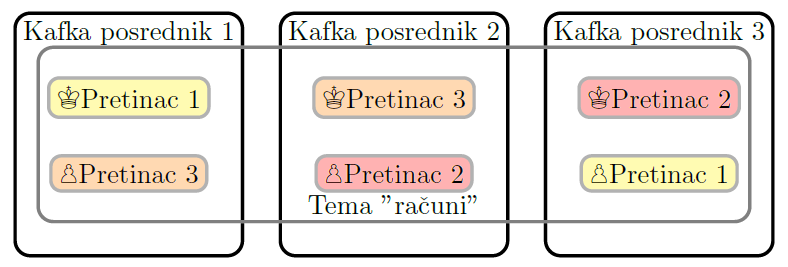
\includegraphics[width=0.8\textwidth]{KafkaPartitions.png}
    \caption{Pretinci vođe i pretinci sljedbenici}
    \label{fig:kafka-leader-follower}
\end{figure}

\ref{fig:kafka-leader-follower} prikazuje tri posrednika u grozdu. Tema "računi" je podijeljena na najveći mogući broj pretinaca: broj posrednika u grozdu. Kako se poruke ne bi izgubile zbog ispada posrednika svaki pretinac teme je umnožen jednom. Vođa žutog pretinca je nasumično posrednik jedan. Vođa crvenog pretinca će biti ili posrednik dva ili tri jer se vodstvo pretinaca mora jednoliko raspodijeliti. Ako vođa crvenog pretinca postane posrednik tri, onda će vođa narančastog pretinca postati posrednik dva. Pretinac pratitelji se ravnomjerno rasporede po posrednicima tako da pratitelji nikad nisu zajedno s vođom u istom posredniku.

Osim sto vođa pretinca je jedini posrednik koji može čitati ili pisati poruke iz pretinca, on se mora brinuti o pratiteljima. Vođa smatra da je pratitelj živ samo ako je prijavljen u Kafka grozd i ako ne zaostaje s čitanjem poruka iz pretinca vode. Ako zaostaje, vođa će pratitelja izbaciti iz skupa usklađenih pratitelja (ISR). Kada vođa primi poruke od objavljivača on će poruke zapisati u svoju particiju i čekat će potvrde pratitelja. Tek kada svi pratitelji pročitaju i zapišu poruke u svoj pretinac će vođa pretinca poslati potvrdu objavljivaču. Pretplatitelji mogu čitati samo one poruke koje su i vođa i pratitelji zapisali u svoje pretince.

Ako se posredniku koji je vođa pretinca dogodi ispad, nitko neće moći čitati ili pisati poruke u pretinac. Zato će pratitelji glasati tko će od pratitelja postati novi vođa pretinca. Samo pratitelji koji su u skupu ukradenih pratitelja mogu postati novi vođa. U iznimnom slučaju kada ne postoji usklađeni pratitelj neusklađeni pratitelj može postati novi vođa pretinca.

Posrednika, tema, pretinaca i umnoženih pretinaca je puno. Kako posrednici ne bi glasali za novog vođu pretinca za svaki pretinac zasebno jedan od posrednika je zadužen da bude nadglednik glasanja. Ako se dogodi ispad posrednika, nadglednik glasanja će ubrzati glasanje novog vođe pretinca.

\subsection{Pretplatnik}

\begin{figure}[H]
    \centering
    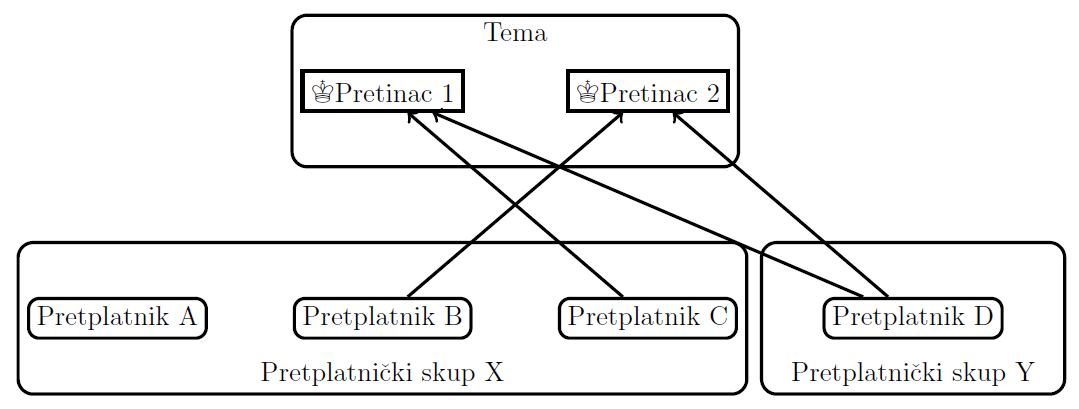
\includegraphics[width=0.8\textwidth]{KafkaConsumerGroups.png}
    \caption{Kafka pretinci i skup pretplatnika}
    \label{fig:kafka-consumer-group}
\end{figure}

Pretplatnik je korisnički program koji čita poruke iz teme. \ref{fig:kafka-consumer-group} prikazuje odnos pretplatnika i teme. Svaki pretplatnik je član samo jedne skupine pretplatnika. Skupina pretplatnika sastojati se od barem jednog člana. Skupina pretplatnika zajedno čita poruke iz teme. Neki pretplatnici u skupu pretplatnika biti će zaduženi za čitanje poruka iz teme. Svaki zaduženi pretplatnik ima barem jedan pretinac iz kojeg jedino on može čitati poruke. Skupina pretplatnika može istovremeno napraviti najviše P čitanja ako je P broj pretinaca i u skupini pretplatnika je barem P članova. Poruke se mogu pročitati jedino iz pretinca vođe. Ako pretplatnik uputi zahtjev za čitanje pratitelju pretinca on će pretplatnika preusmjeriti na vođu pretinca.

Pretplatnik u zahtjevu za čitanje navodi odmak zadnje pročitane poruke i koliko poruka želi pročitati. Posrednik će dostaviti sve poruke od odmaka do tražene količine ili dok ne dođe do kraja pretinca. Odmak poruke je i jedinstvena oznaka poruke i mjesto u datoteci posrednika gdje se poruka nalazi. Posrednik ne pazi koje je poruke pretplatnik pročitao. Pretplatnik je zadužen za rukovanje odmakom. Odmak zadnje pročitane poruke pretplatnik šalje u posebnu temu posrednika. Ako se dogodi ispad pretplatnika, drugi pretplatnik će pročitati odmak iz teme i nastaviti s čitanjem poruka iz pretinca.

Posrednik će jednom pretplatniku po skupini pretplatnika dostaviti poruku barem jednom. Ako se dogodi ispad pretplatnika ista poruka se može dostaviti više puta. Ako je nedopustivo istu poruku pročitati više puta onda korisnik mora napraviti vlastiti algoritam ili koristiti transakcijskog pretplatnika. Pretplatnik čita poruke onim redoslijedom kojim su poruke zapisne u pretinac. Posrednici vremenski ne uređuju dostavu poruka iz svih pretinaca, ali su poruke vremenski uređene u svakom pretincu pojedinačno. Ako je potrebno vremenski urediti sve poruke u svim pretincima onda je potrebno razviti vlastiti algoritam ili napraviti temu sa samo jednim pretincem.

Više skupina pretplatnika može istovremeno citati poruke iz iste teme i pretinaca. Posrednik će odaslati istu poruku svim pretplaćenim pretplatnicima. Posrednici će skupu pretplatnika omogućiti čitanje poruka samo ako su svi pratitelji u skupu usklađenih pratitelja i vođa pretinca zapisali poruke u pretinac. Nakon što pretplatnik primi poruke on će u temi odmaka ažurirati odmak do kojeg je pročitao poruke.

Model povlačenja poruka pretplatnicima dopušta čitanje poruka brzinom koja njima odgovara. Model dopušta i učinkovito razašiljanje iste poruke na više pretplatnika. Ako pretplatnik želi ponovno pročitati poruku on samo treba poslati odmak pročitane poruke. Kako pretplatnik ne bi zaglavio u petlji ako u pretincu nema novim poruka on sebe može blokirati dok ne dođu nove poruke. Posrednik nikad ne zna kada su svi pretplatnici pročitali poruke i zato ih ne može obrisati nakon čitanja. Posrednici su zato napravljeni da s povećanjem nepročitanih poruka njihova učinkovitost ne opada. Posrednik će poruke izbrisati nakon zadanog vremena.

\section{Apache Pulsar}

\begin{figure}[H]
    \centering
    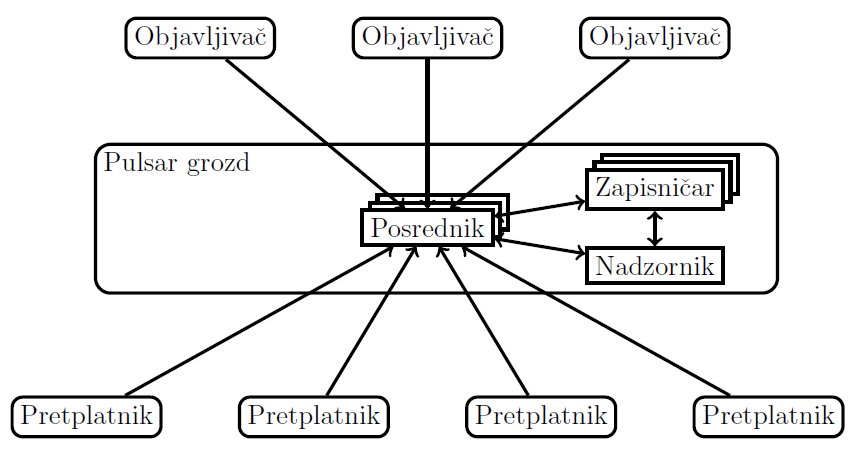
\includegraphics[width=0.8\textwidth]{PulsarCluster.png}
    \caption{Apache Pulsar grozd}
    \label{fig:pulsar-cluster}
\end{figure}

Apache Pulsar je moderni alat za raspodijeljenu obradu tokova podataka. \ref{fig:pulsar-cluster} prikazuje Pulsar proces koji se sastoji od barem jednog Pulsar grozda. Pulsar grozd sastoji se od barem jednog Pulsar posrednika, od barem jednog Apache BookKeeper zapisnicara i Apache ZooKeeper nadzornika. Objavljivači šalju poruke u temu grozda. Posrednici primaju i posluzuju poruke, a zapisnicari ih zapisuju. Pretplatnici čitaju poruke iz teme grozda i obrađuju podatke. \citep{pulsar-docs} \citep{pulsar-streamlio-1} \citep{pulsar-streamlio-2} \citep{pulsar-streamlio-intro} opisuju primjenu, arhitekturu i izvedbu Pulsar pretplatnika, upravljane knjige, posrednika, teme, pretplate i objavljivača.

\subsection{Objavljivač}
Objavljivač je korisnički program koji šalje poruke u temu. Poruke se nužno sastoje od sadržaja, oznake objavljivača, jedinstvene oznake poruke i vremena objave. Poruke se mogu slati u skupini. Prije slanja, poruke se mogu sažeti. Tema može biti podijeljena na pretince. Objavljivač može usmjeriti poruke u određeni pretinac. Poruke se mogu usmjeriti na jedan nasumični pretinac, na točno određene pretince koristeći ključ ili se mogu slati jednoliko na sve pretince. Objavljivači ili čekaju potvrdu dok posrednik zapisuje poruke ili nastave s radom i naknadno provjere je li su poruke primljene i zapisane.

\subsection{Tema i pretplata}

\begin{figure}[H]
    \centering
    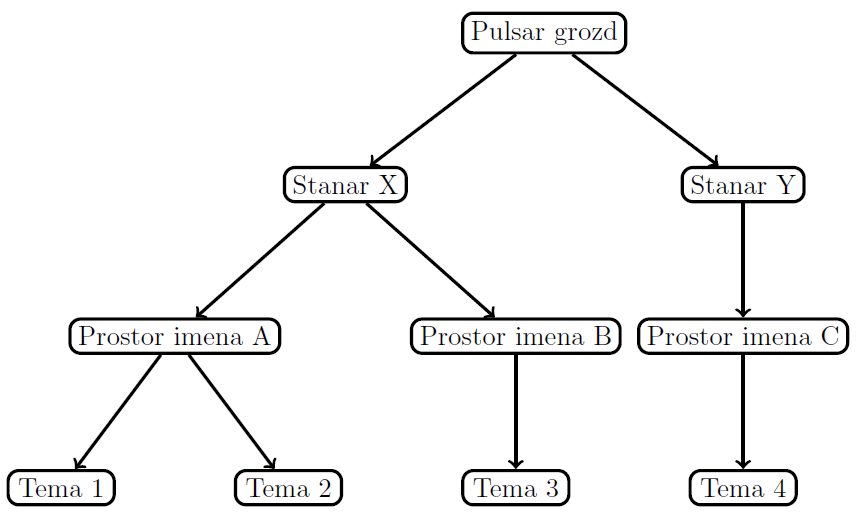
\includegraphics[width=0.8\textwidth]{PulsarHierarchy.png}
    \caption{Pulsar teme, prostori imena i stanari}
    \label{fig:pulsar-hierarchy}
\end{figure}

Tema je imenovani tok poruka koji prenosi poruke od objavljivača do pretplatnika kroz posrednika. Tema je izgrađena kao poveznica. \ref{fig:pulsar-hierarchy} prikazuje stupnjevanje tema, prostor imena i stanara. Svaka tema pripada jednom prostoru imena. Prostor imena je upravna jedinka kojom se mijenjaju postavke tema. Svaki prostor imena pripada jednom stanaru. Stanar određuje način pristupa, korištenje resursa, brisanje poruka i izolaciju prostora imena. Stanari pripadaju Pulsar grozdu.

\begin{figure}[H]
    \centering
    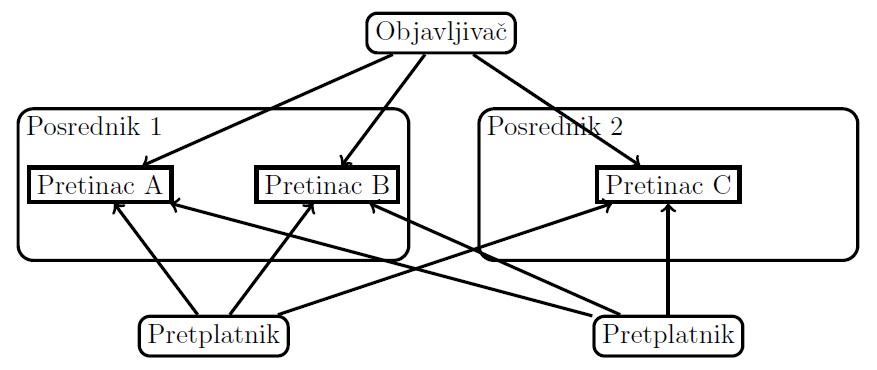
\includegraphics[width=0.8\textwidth]{PulsarPartitions.png}
    \caption{Pulsar pretinci}
    \label{fig:pulsar-partitions}
\end{figure}

Moguće je napraviti bezmemorijske teme koje poruke čuvaju do slanja pretplatnicima ili ispada posrednika. Bezmemorijske teme objavljene poruke potiskuju prema pretplatnicima. Prednost bezmemorijskih tema je brzina. Količina nepročitanih poruka u temi ne utječe na protok poruka kroz temu. Poruka se briše iz teme kada svi pretplatnici pročitaju poruku ili kada je poruka pročitana i starija od zadane vrijednosti ili kada je nepročitana i starija od zadane vrijednosti. Tema se može podijeliti na više podtema zvanih pretinac. \ref{fig:pulsar-partitions} prikazuje odnos objavljivača i pretplatnika prema temi koja je podijeljena na pretince. Pretinci su ravnomjerno raspodijeljeni po posrednicima. Broj istovremenih pretplatnika odnosno čitanja nije ograničeno brojem pretinaca.

\begin{figure}[H]
    \centering
    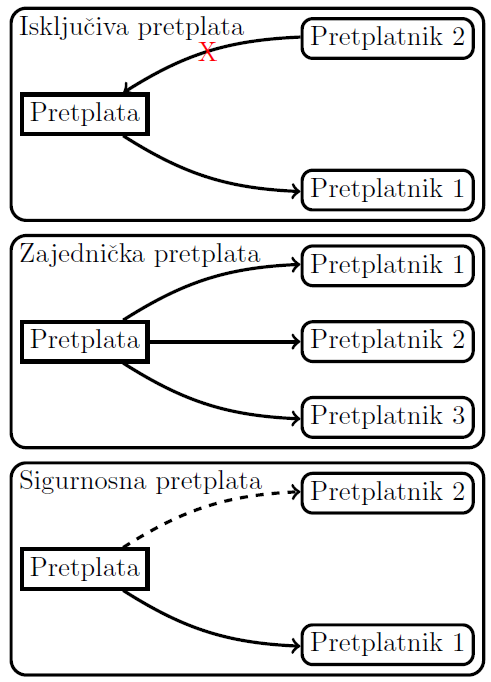
\includegraphics[width=0.5\textwidth]{PulsarSubscription.png}
    \caption{Pulsar pretplate}
    \label{fig:pulsar-subscription}
\end{figure}

Kako objavljivači usmjeravaju dostavu poruka na pretince tako pretplatnici čitaju poruka koristeći pretplate. \ref{fig:pulsar-subscription} prikazuje tri vrste pretplata. Isključiva pretplata pravo čitanja poruka daje samo jednom pretplatniku. Ako drugi pretplatnik pokuša čitati iz isključive pretplate on će biti odbijen. Zajednička pretplata jednoliko dostavlja poruke pretplatnicima. Svaka poruka dostavit će se samo jednom pretplatniku. Zajednička pretplata ne podržava skupnu potvrdu dostave poruka niti pazi na vremensko uređenje dostave poruka. Sigurnosna pretplata pravo čitanja daje samo jednom pretplatniku dok se pretplatniku ne dogodi ispad. Kada se dogodi ispad drugotni pretplatnik će nastaviti čitanje poruka od mjesta ispada.

\subsection{Posrednik}
Posrednik je program bez stanja koji se sastoji od dva dijela. Prvi dio je poslužitelj s REST sučeljem za upravljanje i pretraživanje tema, a drugi dio je otpravnik za prijenos podataka. Umjesto da objavljivači i pretplatnici izravno razgovaraju s posrednikom mogu se spojiti na zastupnika koji će preusmjeriti njihove zahtjeve posrednicima. Posrednik može odbaciti udvostručene poruke tako da ih ne proslijedi zapisničarima.

Pulsar grozdovi mogu umnožiti poruke ako pripadaju istom procesu. Zadaća posrednik je poslužiti poruke pretplatnicima iz upravljane knjige ili BookKeeper zapisničara, dok je ZooKeeper nadzornik zadužen za čuvanje podata o grozdu. Zapisničar zapisuje poruke koje su poslane posredniku.

\subsection{Upravljana knjiga}
BookKeeper grozd je raspodijeljeni zapisivač koji se sastoji od barem jednog zapisničara. Zapisničar zapisuju poruke koje mu posrednici pošalju. Poruke se mogu umnožiti i zapisati u više knjiga odjednom. Svaka tema sastoji se od barem jedne knjige. Kapacitet poruka koji može se povećati dodavanjem zapisničara. Zapisničari mogu istovremeno čitati i pisati poruke.

Knjiga je struktura podatka u koju se poruke mogu dodati samo na kraj. Nakon što se knjiga zatvori ona se jedino može čitati. Ako se zapisničaru dogodi ispad, knjiga se zatvori. Kada se ispad otkloni zapisničar će ustanoviti u kojem je stanju knjiga i ustanovljeno stanje poslati ostalim zapisničarima u grozdu.

Upravljana knjiga je skup BookKeeper knjiga u koju se upisuju poruke koje pripadaju jednoj temi. Iako se poruke mogu zapisati u samo jednu knjige više BookKeeper knjiga olakšava brisanje i pisanje poruka. Upravljana knjiga sastoji se skupa tokova podata koji se zapisuju u knjigu s jednim pisaćem i skupa pokazivača koji prate koje poruke su pretplatnici pročitali. Zapisivač prije pisanja poruke u upravljanu knjigu poruke zapisuje u dnevnik.

\subsection{Pretplatnik}
Pretplatnik je korisnički program koji se pretplaćuje na pretplatu teme. Postoje tri vrste pretplate. Svaka pretplata određuje način na koji pretplatnik čita poruke. Pretplatnik može ili biti blokiran dok posrednik ne dobije poruku ili nastaviti s radom i dobiti budućnosnicu kojom će čitati poruke. Pretplatnik može pojedinačno ili skupno potvrditi poruke.

Ako korisnik nije zadovoljan izvedenim pretplatnikom on može koristiti sučelje čitača. Sučelje čitača je biblioteka koja omogućuje ručno potvrđivanje poruka, ponovno čitanje poruke i odbacivanje umnoženih poruka.

\section{RabbitMQ}

\section{Usporedba}

\begin{table}[]
\begin{tabular}{lllll}
 &  &  &  &  \\
 &  &  &  &  \\
 &  &  &  &  \\
 &  &  &  & 
\end{tabular}

\caption{Text below table}
\label{table:sample_table_label}

\end{table}

\chapter{Specifikacija sustava}

Apache Kafka živi u okruženju s drugim sustavima. Okruženje je opisano pretpostavkama koje su nepromjenjive i uvijek vrijede. Zahtjevi su poželjna svojstva i mogućnosti programa koji mogu ali ne trebaju biti ispunjeni.

\section{Pretpostavke}

\begin{itemize}
    \item Nadzirani sustav i sakupljač vrijednosti koriste siguran intranet
    \item Postoji više od deset Kafka grozdova i više od sto Kafka posrednika
    \item Kafka posrednici raspodijeljeni su na velik broj računala
    \item Kafka grozdovi i posrednici mogu se upaliti i ugasiti u bilo kojem trenutku
    \item Može se dogoditi ispad, ali ne i bizantski
\end{itemize}

\section{Zahtjevi}

\begin{itemize}
    \item Sakupljač vrijednosti se lako umnoži i nije pozadinski proces
    \item Sakupljač vrijednosti samostalno pronalazi nove Kafka grozdove i posrednike
    \item Sakupljač vrijednosti šalje nadzirane vrijednosti s malim zakašnjenjem od trenutka očitavanja
    \item Sakupljač vrijednosti očitava nadzirane vrijednosti svake sekunde ili češće
    \item Sakupljač vrijednosti zapisuje nadzirane vrijednosti u Kafka temu
    \item Sakupljač vrijednosti oslobađa računalne resurse kada se nadzirani sustav ugasi
    \item Nadzirane vrijednosti imaju jedinstvenu oznaku nadziranog sustava iz kojeg su pročitane
    \item Nadzirane vrijednosti imaju vremensku oznaku kada su pročitane
\end{itemize}

\chapter{Postojeća rješenja}

Istraživanje postojećih rješenja ima višestruku ulogu: odrediti mane i prednosti izvedenog rješenja nad postojećim; naučiti zašto i kako su drugi riješili problem; ponovno iskoristiti ili unaprijediti postojeće rješenje. U nadi da postoji rješenje koje zadovoljava većinu ili sve zahtjeve sustava istraženi su mali programi i veliku sustavi.

\section{Jolokia}

\begin{figure}[H]
    \centering
    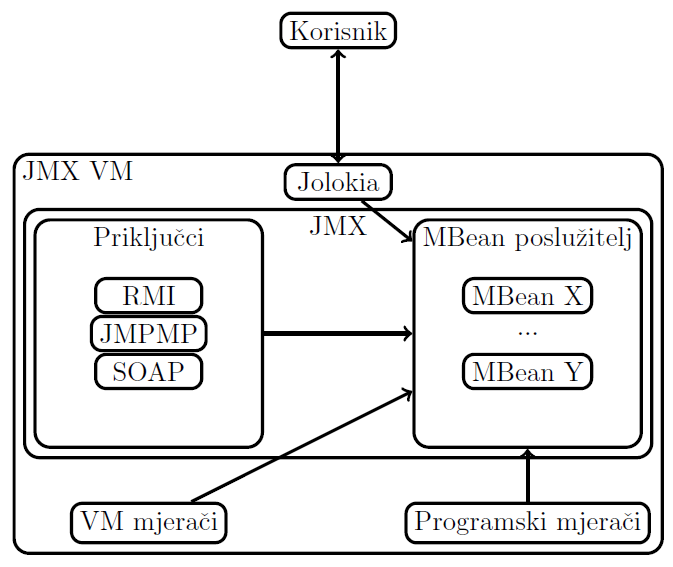
\includegraphics[width=0.8\textwidth]{Jolokia.png}
    \caption{Arhitektura Jolokie}
    \label{fig:jolokia}
\end{figure}

Jolokia je u \citep{jolokia} opisana kao most između JMX i HTTP. Jolokia se pokreće kao agent u Java VM ili kao samostojeći poslužitelj. \ref{fig:jolokia} prikazuje izvršavanje upita. HTTP upit postavi se Jolokiji koja skriva komplicirano dobavljanje nadziranih vrijednosti iza jednostavne funkcije. Nadzirane vrijednosti Jolokia šalje korisniku u JSON obliku.

Jolokia je vrlo jednostavno i krepko rješenje za nadziranje Java programa. Nažalost, Jolokia krši zahtjeve pozadinskog procesa i samostalnog pronalaženja novih Kafka grozdova i posrednika. Ako se Jolokia pokrene kao agent ona se pokrene kao poseban pozadinski proces na računalu na kojem se nalazi nadzirani sustav. Ako se pokrene kao samostojeći poslužitelj ona neće znati kada se upalio novi Kafka grozd ili posrednik jer nema načina da Jolokiji dojave da postoje.

\section{Prometheus}

\begin{figure}[H]
    \centering
    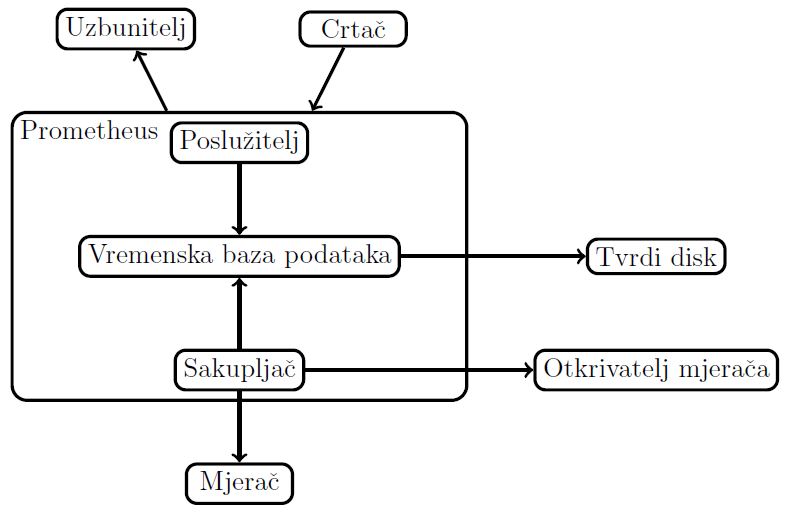
\includegraphics[width=0.8\textwidth]{Prometheus.png}
    \caption{Arhitektura Prometheusa}
    \label{fig:prometheus}
\end{figure}

Prometheus je u \citep{prometheus} opisan kao potpuno rješenja za nadziranje proizvoljnih programa. \ref{fig:prometheus} prikazuje dijelove Prometheusa: poslužitelj, vremenska baza podataka i sakupljač nadziranih vrijednosti. Sakupljač mjerače nalazi samostalno ili koristi otkrivatelja. Kada sakupljač pročita vrijednosti one se pohrane u bazu podataka i u stalnu memoriju. Prije prikazivanja ili stvaranja uzbune korisnici mogu izabrati podskup vrijednosti jezikom PromQL koji je nalik SQLu.

Velika prednost i nedostatak Prometheusa je njegov opseg. Problem zahtjeva samo nadzor ne i predočavanje i obradu i zapisivanje podataka. Prometheus također dugo čeka između očitanja nadziranih vrijednosti. Zahtjev traži čitanje svakih sekundu ili manje, a Prometheus čeka par sekundi.

\section{Confluent sakupljač vrijednosti}

Confluent sakupljač vrijednosti je u \citep{confluent-metrics-reporter} opisan kao dodatak na Kafka grozd i posrednika. Sakupljač čita i šalje nadzirane vrijednosti u Kafka temu nadziranog ili nekog drugog grozda. Svi novi Kafka posrednici pokreću se s Confluent sakupljačem.

Confluent sakupljač vrijednosti ispunjuje sve zahtjeve. Nije pozadinski proces jer dolazi u obliku JAR datoteke koja se veže na, pali se i gasi s Kafka grozdom i posrednikom i šalje nadzirane vrijednosti visokom frekvencijom. Nažalost, Confluent sakupljač vrijednosti je zatvoreno rješenje koje se ne može nadograditi, poboljšati ili proširiti.





\chapter{Arhitektura sustava}

\citep{clean-code} \citep{code-complete} opisuju kako oblikovati programski sustav. Sustav se oblikuje na razini okoline, rješenja, projekta, klase, funkcije i naredbe. Okolina je skup pretpostavka o računalu, operacijskom sustavu, postojećim sustavima i mreži. Rješenje je skup projekata koji zajedno rješavaju problem. Projekt je program koji ispunjava podskup zahtjeva sustava. Klasa je skup podatka i funkcija koje djeluju nad njima u objektno orijentiranoj paradigmi, a skup funkcija u proceduralnoj paradigmi.

\section{Okolina}

\begin{figure}[H]
    \centering
    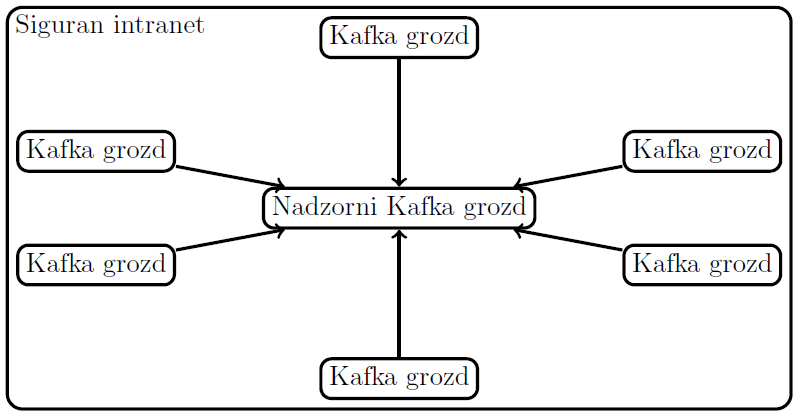
\includegraphics[width=0.8\textwidth]{KafkaEnvironment.png}
    \caption{Okolina sustava}
    \label{fig:kafka-environment}
\end{figure}

\ref{fig:kafka-environment} prikazuje mali podskup Kafka grozdova. Grozdovi koriste sigurni intranet za međusobni razgovor. Napadač ne postoji i ne može izazvati ispad pogrešnim korištenjem programa. Grozd može iskusiti ispad. Kafka grozdovi se mogu se upaliti i ugasiti u bilo kojem trenutku. Dijelovi grozda raspodijeljeni su na više računala. Kafka grozdovi šalju nadzirane vrijednosti u središnji nadzorni Kafka grozd. Nadzorni grozd je otporan na ispade i fizički odvojen od ostalih grozdova.

\section{Arhitektura rješenja}

\begin{figure}[H]
    \centering
    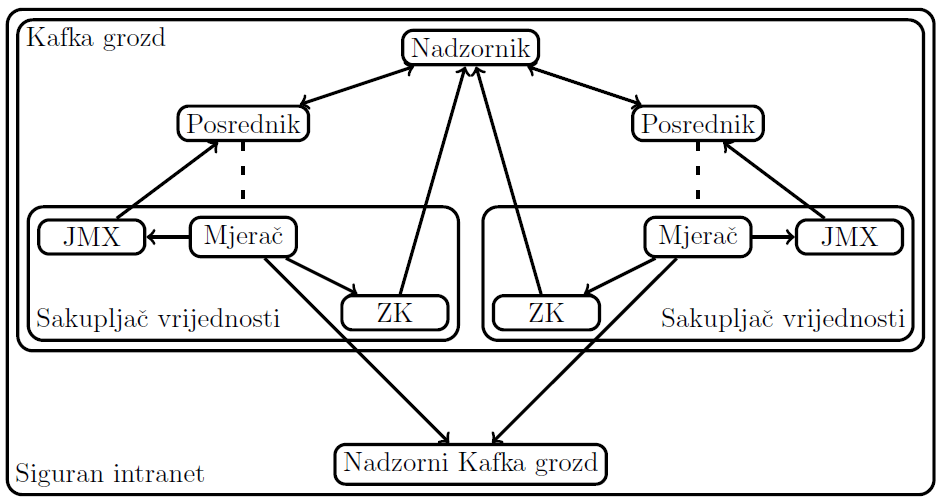
\includegraphics[width=0.8\textwidth]{KafkaCollectors.png}
    \caption{Nadzor jednostavnog Kafka grozda}
    \label{fig:collectors}
\end{figure}

\ref{fig:collectors} prikazuje kako sakupljači vrijednosti nadziru Kafka posrednike. Kafka grozd sastoji se od barem jednog Kafka posrednika i ZooKeeper nadzornika. Posrednici šalju poruke pretplatnicima i zapisuju poruke objavljivača. Nadzornik zapisuje podatke o grozdu. Svaki posrednik ima svog sakupljača vrijednosti. Kada se pokrene posrednik pokrene se i sakupljač vrijednosti. Sakupljač vrijednosti sastoji se od tri projekta: mjerača, ZK i JMX. Mjerač pita ZK kojeg posrednika treba nadzirati. Zatim mjerač od JMX saznaje nadzirane vrijednosti. Svi mjerači šalju nadzirane vrijednosti u udaljeni nadzorni Kafka grozd.

\section{Arhitektura projekt}

Rješenje je podijeljeno na projekte gdje svaki ispunjuje disjunktni podskup zahtjeva sustava. Projekti se mogu nadograditi i ispraviti bez utjecaja na druge projekte. U projektu od nekoliko klasa je lakse naći grešku nego u velikom projektu. Projekte je primjereno izvesti na objektno orijentirani nacin. Svaka klasa zadužena je za jednu domenu problema.

\subsection{Arhitektura ZK}

\begin{figure}[H]
    \centering
    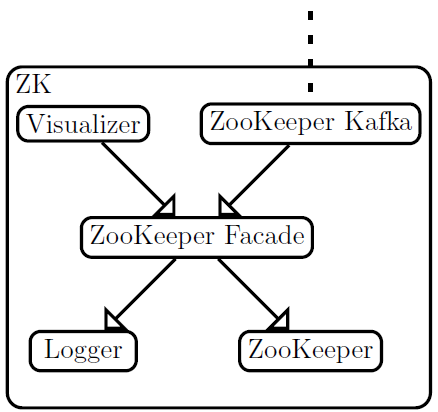
\includegraphics[width=0.8\textwidth]{ZooKeeperKafka.png}
    \caption{}
    \label{fig:zookeeper-kafka}
\end{figure}

\begin{itemize}
    \item Visualizer zadužen za predocavanje podataka zapisanih u ZooKeeper nadzorniku
    \item ZooKeeper Kafka zadužen za apstrahiranje odnosa Kafka posrednika i ZooKeeper nadzornika
    \item ZooKeeper Facade zadužen za razgovor s ZooKeeper nadzornikom
    \item Logger zadužen za ispisivanje događaja
    \item ZooKeeper zadužen za izvršavanje ZooKeeper naredba
\end{itemize}

\subsection{Arhitektura JMX}

\begin{figure}[H]
    \centering
    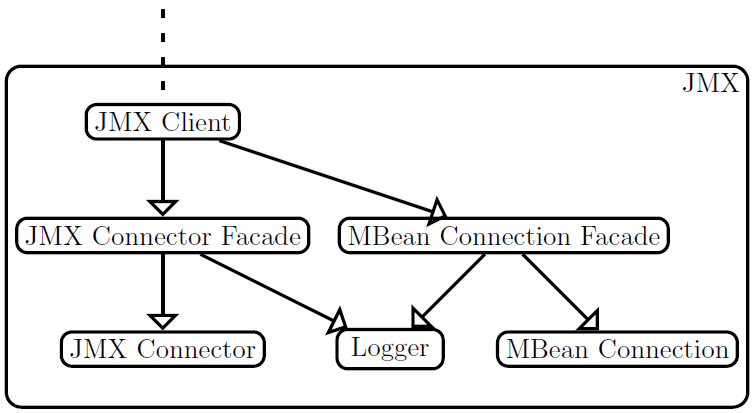
\includegraphics[width=0.8\textwidth]{JMXClient.png}
    \caption{}
    \label{fig:jmx-client}
\end{figure}

\begin{itemize}
    \item JMX Client zadužen za apstrahiranje JMX sustava
    \item JMX Connector Facade zadužen za spajanje s JMX uslugama
    \item MBean Connection Facade zadužen za očitavanje MBean vrijednosti
    \item JMX Connector zadužen za izvršavanje JMX naredba
    \item Logger zadužen za ispisivanje događaja
    \item MBean Connection zadužen za izvršavanje MBean naredba
\end{itemize}

\subsection{Arhitektura mjerača}

\begin{figure}[H]
    \centering
    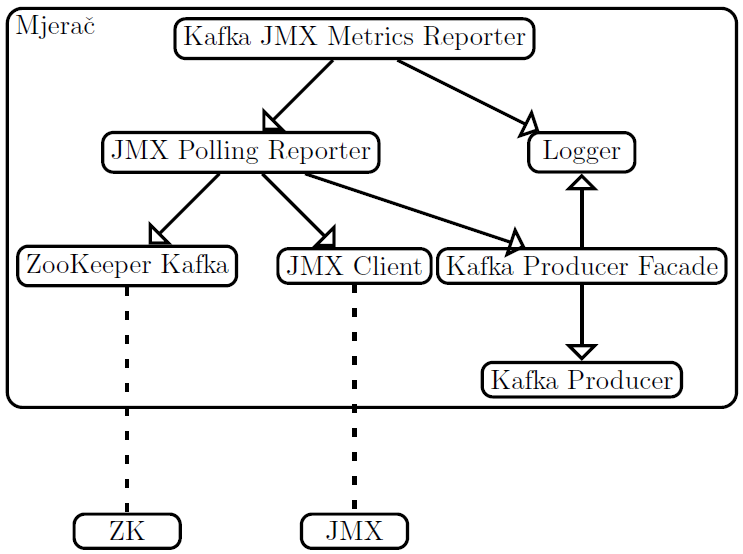
\includegraphics[width=0.8\textwidth]{KafkaMetricsReporter.png}
    \caption{}
    \label{fig:kafka-metrics-reporter}
\end{figure}

\begin{itemize}
    \item Kafka JMX Metrics Reporter zadužen za pokretanje sakupljača vrijednosti
    \item JMX Polling Reporter zadužen za očitavanje nadziranih vrijednosti
    \item Logger zadužen za ispisivanje događaja
    \item ZooKeeper Kafka zadužen za apstrahiranje odnosa Kafka posrednika i ZooKeeper nadzornika
    \item JMX Client zadužen za apstrahiranje JMX sustava
    \item Kafka Producer Facade zadužen za 
    \item Kafka Producer zadužen za objavu nadziranih vrijednosti u Kafka temu
\end{itemize}

\chapter{Izvedba}

\section{Izvebda rješenja}

Rješenje je izvedeno u programskom jeziku Java 8 za programske alate Apache Kafka 2.1 i Apache ZooKeeper x.x. Za projektno upravljanje koristi se Apache Maven, a programska okolina je ostvarena s Eclipse X. Rješenje se pakira u .jar datoteku koristeci Maven. Koriste se X i Y Maven plugin.  .jar se mora stviti u datoteku /libs u Kafki. Potrebno je pazljivo pakirati pomocne biblioteke jer se mogu sukobiti ovisnosti. Upute kako koristiti i postaviti program su dane u prilogu.

Stil pisanja i nacin imenovanja je definiran u Google Java Style. 

Funkcje su vrlo kratke, samo nekoliko redova dugacke. Srednji broj redova je X. Super super detalji slijede!

\section{Izvebda projekta}

\section{Izvebda paketa}

\section{Izvebda klase}

\section{Izvebda funkcije}

\section{Izvebda naredbe}

Programske naredbe dijele se na izraze i izjave. Izjave ne vraćaju vrijednost, dok izrazi vraćaju. 

Varijable se mogu imenovati ili iz rijecnika domene problema ili iz rijecnika racunalne znanosti. !CITAT tvrdi da ..., dok !CITAT tvrdi da ....



Razina okoline
Razina rješenja
Razina projekta
Razina paketa
Razina klase
Razina funkcije
Razina naredbe

\section{Kafka Connect}

\begin{figure}[H]
    \centering
    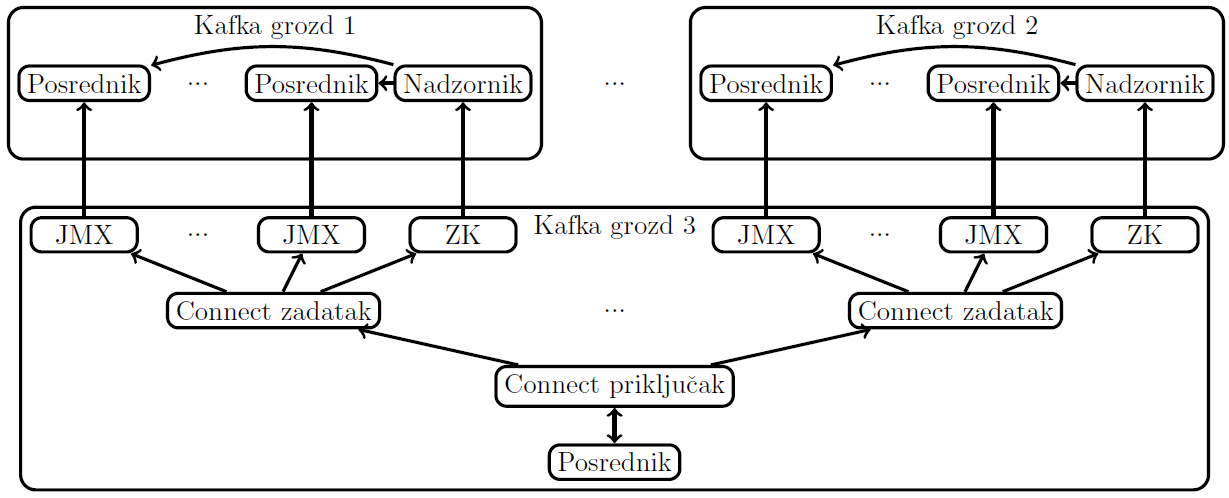
\includegraphics[width=0.8\textwidth]{KafkaConnect.png}
    \caption{Arhitektura Kafka Connect sakupljača vrijednosti}
    \label{fig:kafka-connect}
\end{figure}

Kafka Connect je u !CITAT opisana kao alat za razmjenu podataka izmedu Apache Kafke i vanjskog sustava. Kafka Connect sastoji se od priključka koji stvara odredeni broj paralelnih zadataka. Kafka Connect dijeli se na Source Connect koji upisuje poruke u Kafku i Sink Connect koji cita poruke iz Kafke.

Kafka Connect nemoze otkriti nove Kafka grozdove i posrednike jer ne sustava za prijavu.

\chapter{Rezultati}

\chapter{Zaključak}
Zaključak.

\chapter{Prilog}

\section{Priručnik za korištenje}
\begin{lstlisting}[breaklines]
## Kafka Metrics User Guide

This guide will go through all the steps necessary to configure and run KaSta Pull and Push projects.  

All examples and commands assume you are working with CentOS 7 operating system.



### Preparing Kafka environment

You need to configure your environment at the hardware, operating system and application level.  

#### [Hardware](https://kafka.apache.org/documentation/#hwandos)

Your machine needs to have sufficient memory to run Kafka.  
I advise at least 4GB of RAM.  

#### [OS](https://kafka.apache.org/documentation/#os)

Kafka should work well on any Unix system and is tested on both Linux and Solaris.  
Avoid running Kafka on Windows.  

#### [Java version](https://kafka.apache.org/documentation/#java)

Kafka requires Java Development Kit (JDK) 1.8 or better to run.  
```
$: sudo yum install java
```



### Installing Kafka

After preparing the environment you are ready to install Kafka.  
I strongly advised you install Kafka in the [/opt directory](https://www.tldp.org/LDP/Linux-Filesystem-Hierarchy/html/opt.html).  

Download Kafka:  
```
$: sudo curl "https://www.apache.org/dist/kafka/2.1.1/kafka_2.11-2.1.1.tgz" -o /opt/kafka.tgz
```

Install Kafka:  
```
$: cd /opt/kafka
$: sudo mkdir kafka
$: sudo tar -xvzf /opt/kafka.tgz --strip 1
```

Uncomment a property in Kafka's server.properties:  
```
listeners=PLAINTEXT://:9092
```



### Running Kafka

Start Zookeeper:  
```
$: sudo bin/zookeeper-server-start.sh config/zookeeper.properties
```

Start Kafka and open the JMX port:  
```
$: sudo JMX_PORT=Any-Free-Port bin/kafka-server-start.sh config/server.properties
```



### Preparing KaSta environment

#### [Git](https://git-scm.com/)

Install Git:  
```
sudo yum install git
```

#### [Maven](http://maven.apache.org/)

Install Maven:  
```
sudo yum install maven
```

#### Supporting projects

Download JMX Client:
```
$: cd /opt/projects
$: sudo git clone JMX-Client-Project-URL jmx-client
```

Download Zookeeper Client:
```
$: cd /opt/projects
$: sudo git clone ZK-Client-Project-URL zk-client
```

Install both projects with Maven:
```
$: cd /opt/projects/jmx-client
$: sudo mvn install

$: cd /opt/projects/zk-client
$: sudo mvn install
```



### Installing KaSta

Download KaSta Pull Connect:  
```
$: cd /opt/projects
$: sudo git clone KaSta-Pull-Project-URL kasta-pull
```

Download KaSta Push Reporter:  
```
$: cd /opt/projects
$: sudo git clone KaSta-Push-Project-URL kasta-push
```

Package KaSta Pull Connect into a JAR:  
```
$: cd /opt/projects/kasta-pull
$: sudo mvn package
```

Package KaSta Push Reporter into a JAR:  
```
$: cd /opt/projects/kasta-push
$: sudo mvn package
```

KaSta Push will make a JAR that will contain only dependencies on JMXClient and Zookeeper Client.

```
<artifactId>maven-shade-plugin</artifactId>
  <version>3.2.1</version>
    <configuration>
      <artifactSet>
        <includes>
          <include>mjaksic:zookeeper-client</include>
          <include>mjaksic:jmx-client</include>
        </includes>
      </artifactSet>
    </configuration>
...
```

Otherwise, if a fully fat JAR is made, it will crash because of dependency conflict with other JARs in Kafka's `libs/` dir

### Configuring KaSta Pull Connect

KaSta Pull Connect JAR must be placed into /opt/connectors folder.
```
$: sudo cp /opt/projects/kasta-pull/target/kafka-jmx-connect.jar /opt/connectors/
```

Optionally, review Connector properties in /opt/projects/kasta-pull/target.



### Configuring KaSta Push Reporter

KaSta Push Reporter JAR must be placed into Kafka's /libs folder.
```
$: sudo cp /opt/projects/kasta-push/target/kafka-jmx-reporter.jar /opt/kafka/libs/
```

Append to Kafka's server.properties:
```
kafka.metrics.reporters=mjaksic.kafka_jmx_reporter.broker.KafkaJMXMetricsReporter
```

Optionally, these properties may be appended as well:
```
reporter.delay.milliseconds=5000
reporter.interval.milliseconds=1000
metrics.kafka=localhost:9092
kafka.metrics.topic=jmx-metrics
```



### Running KaSta Pull Connect

After starting Kafka run:  
```
sudo /opt/kafka/bin/connect-standalone.sh /opt/kafka/config/connect-standalone.properties /opt/projects/kasta-pull/target/connector-config.properties
```



### Running KaSta Push Reporter

The Reporter is run when you run Kafka. That's it!  



### Supplementary guides

* [Official Kafka Quickstart](https://kafka.apache.org/quickstart)

* [DigitalOcean: Install Kafka on CentOS 7](https://www.digitalocean.com/community/tutorials/how-to-install-apache-kafka-on-centos-7)

\end{lstlisting}

\bibliography{literatura}
\bibliographystyle{fer}

\begin{sazetak}
Sažetak na hrvatskom jeziku.

\kljucnerijeci{Ključne riječi, odvojene zarezima.}
\end{sazetak}

\engtitle{Real-Time Health Monitoring in Distributed Data Stream Processing System}
\begin{abstract}
Abstract.

\keywords{Keywords.}
\end{abstract}

\end{document}
